\chapter{IVOA structure} % (fold)
\label{cha:the_ivoa}
	
	The International Virtual Observatory Alliance mission and
	high-level structure was described in section
	\ref{sec:the_international_virtual_observatory_alliance} of the
	introduction to the Virtual Observatory.
	
	In this appendix, we provide a detailed overview of the different
	constituents of the IVOA: Working Groups, Interest Groups, and 
	directive committees.
	
	\section{Working Groups} % (fold)
	\label{sec:working_groups}
		
		The existing IVOA Working
		Groups\urlnote{http://www.ivoa.net/intranet/} (IVOA WGs)
		are the following:
		
		\begin{description}
			\item[Applications] This WG is devoted to VO
			application development. Group members have specified
			several application interoperability protocols (first
			PLASTIC, the PLatform for AStrophysical Tool
			Interoperability and Collaboration; later SAMP, the
			Simple Application Messaging Protocol), and used them
			to enable VO data sharing between applications running
			on the same machine.
			
			 \item[Data Access Layer] If we view the VO as a
			superposition of layers which provide services to the
			layers above them, the Data Access Layer would be the
			one allowing applications to access data by calling VO
			services. In particular, this WG is devoted to the
			development of the data access protocols for the VO.
			The Simple Cone Search~\cite{Williams:2008fv} was the
			first DAL protocol, followed by the
			SIAP~\cite{2008sia..rprt.....T} and the
			SSAP~\cite{Tody:2007yq} protocols\footnote{It should
			be noticed that the SIAP is a protocol still in the
			Working Draft stage, and which is being adapted to
			the common principles used for SSAP.}.
			
			 \item[Data Modelling] This WG deals with the
			domain-specific data models needed to make astronomical
			information interoperable, defining the metadata needed
			for VO queries and automated data mining. The
			Characterisation data model~\cite{McDowell:2007ly} is
			the most successful product of this WG.
			
			 \item[Grid and Web Services] This WG provides the
			liaison between the Virtual Observatory and the grid,
			and other forms of distributed computing. In
			particular, the GWS WG has created a web services
			wrapper, the Common Execution
			Architecture~\cite{Harrison:2005la}, for several data
			mining, processing, and retrieval tasks, so that they
			can be offloaded to more powerful servers for further
			processing. The services themselves can be implemented
			either on standalone machines, or on the grid,
			transparently to the user.
			
			 \item[Resource Registry] This WG is devoted to one of
			the key parts of the VO, the discovery of existing
			services via VO Registries. VO Registries comply with
			the Open Archive Initiative Protocol for Metadata
			Harvesting (OAI-PMH), so that readily available
			solutions exist for VO registries. Metadata harvesting
			allows VO registries to share newly registered entries,
			so that eventually any resource can be found by
			querying any Registry. This WG also maintains the
			Registry of Registries (RofR), a list of OAI-PMH
			endpoints which can be used by harvesting registries
			to know which registries to harvest, and for client
			applications to select between available registries.
			
			 \item[Semantics] This WG is dedicated to the mark-up
			of information so that data columns can be explicitly
			identified by their intended meaning, without needing
			to guess the context.
			
			 \item[VO Event] This WG provides the foundation for
			the VO to deal with transient events, such as Gamma-ray
			Bursts (GRBs), supernovae, lensing of microlensing
			events, transits, et cetera, so that any VOEvent aware
			system can decide whether the event is of interest.
			VOEvent packets~\cite{2006AN....327..775W} carry enough
			space-time coordinates to allow for automatic driving
			and aiming of robotics telescopes.
			
			 \item[VO Query Language] This WG aims to provide a
			universal query language for all table-oriented access
			protocols. Current IVOA protocols are target based,
			while many other astrophysical questions, specially on
			systems built around relational databases, can be
			expressed on terms of relational algebra. VOQL is based
			around SQL, with extensions for spatial regions, object
			cross-matching, and understanding of VO data models and
			semantics. The VOQL, also known as the Astronomical 
			Data Query Language (ADQL) was finally standardised
			in 2008, and is an IVOA
			Recommendation~\cite{2008adql.ivoav0910O}.
			
			 \item[VOTable] This WG has already accomplished the
			standardisation of the VO data format. The VOTable,
			build around an initial XML data format by the
			CDS~\cite{2000ASPC..216...83O}, is already mature
			enough, and the WG will stay dormant after the final
			release of the latest VOTable
			specification~\cite{2004votfdivoav0811O}.
		\end{description}

	% section working_groups (end)

	\section{Interest Groups} % (fold)
	\label{sec:interest_groups}
		
		Apart from the Working Groups, several Interest Groups have
		been formed. The Interest Groups are not part of the key
		IVOA infrastructure, but some of them are born to study
		particular needs of the IVOA, to later move them in
		production, or deciding which particular WG will have the
		responsibility to move development further. Interest Groups
		(IGs) could be seen as Working Group incubators. That was
		the case for the VOEvent interest group, which turned into
		a full-blown WG after all the initial work. This is a list
		of active and dormant IGs.
		
		\newcommand{\millenniumsimurl}[0]
		{http://www.mpa-garching.mpg.de/galform/millennium/}
		
		\begin{description}
			\item[Theory] The Theory IG was born to study how
			different kinds of simulated data could be fit within
			the VO infrastructure. Currently two kinds of efforts
			exist in it: a Numerical Simulations effort,
			concentrated on how to exploit large database-based
			simulations such as the Millennium
			Simulation\urlnote{\millenniumsimurl}; and a
			micro-simulations group, devoted to more specific,
			parameter-based simulations (stellar models, Initial
			Mass Function distributions, et cetera). Within this IG
			the Simple Theoretical Access Protocol
			(STAP)~\cite{2007arXiv0711.2629R}, and the Simple
			Numerical Access Protocol where drafted.
			
			 \item[Data Curation and Preservation] This IG group
			was born recently, and its main aim is to study how to
			perform the long term, sustainable, preservation, and
			curation of data within the Virtual Observatory.
			
			 \item[Open Grid Forum AstroRG] This IG is the liaison
			of the IVOA with the Open Grid
			Forum\urlnote{http://www.ggf.org/}. The GWS WG focuses
			on delivering web-services-based distributed computing
			with an unspecified processing backend, while this IG
			specifically seeks to provide reference grid
			implementations of VO services.
			
			 \item[Radio] This IG was the discussion forum for
			radio astronomy specific provisions within the VO.
			However, this group is now considered dormant, and
			radio specific extensions are discussed within the
			different WGs.
		\end{description}
	
	% section interest_groups (end)

	\section{Steering bodies and committees} % (fold)
	\label{sec:steering_bodies_and_committees}
		
		Additionally to this WGs and IGs, which provide the core
		development work, within IVOA there are several steering
		bodies for its governance:
		
		\begin{description}
			
			\item[IVOA Executive Committee] The IVOA Executive
			Committee is the main steering force of the IVOA, and
			it is formed by the representatives of the different
			national and international VO projects, together with
			the IVOA chair and vice-chair.
			
			 \item[Technical Coordination Group] The TCG is a
			committee formed by the Chairs of the Working and
			Interest Groups as well as the IVOA chairs and
			vice-chairs. It has its own chair, and its role is to
			ensure proper technical coordination amongst the
			various IVOA WGs and IGs, as well as being the liaison
			between them and the IVOA Executive Committee.
			
			 \item[Standing Committee on Standards and Processes]
			After having drafted the processes by which IVOA
			standards were to be defined, the IVOA Standards and
			Processes WG was disbanded. However, from time to time
			the need to reform either approved standards or the
			standardisation process will arise, and in that case
			the role of the Standing Committee on Standards and
			Processes is to review and update IVOA processes in
			response to the needs of the IVOA community.
			
		\end{description}
	
	% section steering_bodies_and_committees (end)
	
	\section{Standard definition process} % (fold)
	\label{sec:standard_definition_process}
		\begin{figure}[tbp]
			\centering
				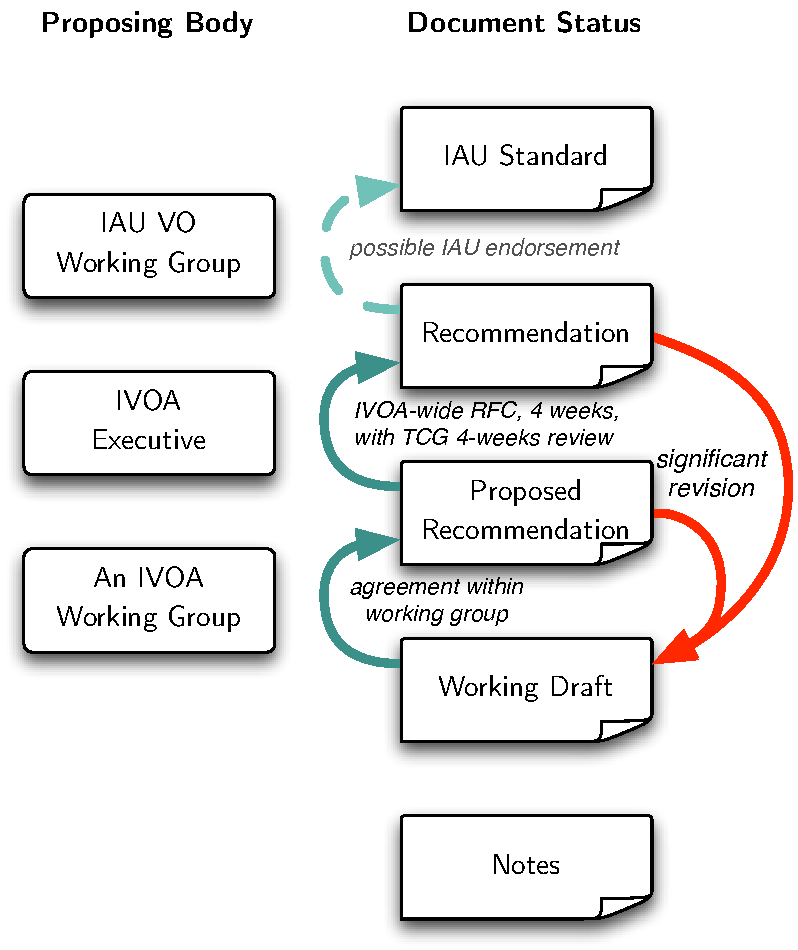
\includegraphics[width=0.66\columnwidth]
				{fig/IVOADocumentProcess.pdf}
			\caption[IVOA Document Process]{
				IVOA Document Process. Standard documents of the
				IVOA can take the form of Working Drafts, Proposed
				Recommendations, and Recommendations, while IVOA
				Notes can be used to publish interesting comments
				on best practices, and might become part of a
				working draft if they are deemed interesting
				enough. IVOA Recommendations are evaluated by the
				IAU VO Working Group, which might propose an IVOA
				Recommendations into a IAU Standard.
			}
			\label{fig:fig_IVOADocumentProcess}
		\end{figure}
		
		IVOA standard documents start their life as Working Drafts
		within any of the existing Working Groups. When a consensus
		has been reached within the Working Group, the Working
		Draft is elevated to the IVOA Executive as a Proposed
		Recommendation, which has to be subject to a four weeks
		review period, or Request For Comments. If no major issues
		have been raised during the RFC review, or by the IVOA
		Executive, the Proposed Recommendation turns into an IVOA
		Recommendation.
		
		 IVOA Recommendations can be later evaluated by the IAU VO
		Working Group in order to become IAU Standards. Currently,
		the only IVOA Recommendation which is an IAU Standard is
		the VOTable data format.
		
		 IVOA Notes can be written by anyone and submitted to a
		suitable working group, but there is no formal process for
		their promotion, other than lobbying in the Working Group
		for the contents of one or several notes to become a
		Working Draft, or part of one.
		
		 In any of the promotion steps the documents MUST
		incorporate the changes agreed within the RFC period, while
		other comments, if duly answered, do not need to be
		incorporated. However, if in any of the stages a
		substantial revision of the document is needed, the
		proposal MUST go back to the Working Draft stage.
		
		This standard promotion process is illustrated in
		figure~\ref{fig:fig_IVOADocumentProcess}, and is documented
		by the \emph{IVOA Document
		Standards}~\cite{2009idstdivoav0302H}.
		
		It should be noted that in the IVOA InterOp meeting of Fall
		2008 in Baltimore, Robert Hanisch announced an agreement
		with the NASA Astronomical Database System, responsible for
		tracking publications related to astronomy. This agreement
		included Working Draft as low-impact refereed publications
		(as Working Drafts need to pass a peer-review among group
		members), while Proposed Recommendations and
		Recommendations will be taking into account as high-impact
		refereed publications (as they have passed an ever tougher
		peer-review process, and will create a IVOA
		Recommendation).
	% section standard_definition_process (end)

% chapter the_ivoa (end)